\chapter{Sufixový strom}\label{chap:sx}

\emph{Sufixový strom} je písmenkový strom pre všetky \emph{sufixy (prípony)} 
daného slova. Jeho veľká výhoda spočíva v rýchlom zostrojení a veľkom množstve 
efektívnych algoritmov na ňom. V softvéri sme vizualizovali jeho zostrojenie, a 
preto ho aj tu popíšeme.

\section{Zostrojenie sufixového stromu}
Existuje veľa spôsobov ako zotrojiť sufixový strom. Najjednoduchšie riešenie 
je využiť písmenkový strom a pridať do neho všetky sufixy. Takéto riešenie má 
časovú aj pamäťovú zložitosť $O(n^2)$. 

\citet{ukkonen} navrhol, ako zostrojiť strom rýchlejšie a za behu. 

\section{Ukkonenov algoritmus}

Hlavnou myšlienkou algoritmu je pre slovo $w_1w_2w_3\cdots w_n\uz$ postupne 
vytvoriť suffixové stromy pre slová $w_1, w_1w_2,\ldots, 
w_1w_2w_3\cdots w_n\uz$. Označme tieto stromy $T(1), T(2),\ldots, T(n), T$. 
Teda, vytvárame $n$ stromov a každý zatiaľ na vytvorenie potrebuje $O(n^2)$ 
krokov. Toto je na prvý pohľad veľmi nešikovné riešenie pretože počet 
krokov potrebných na zostrojenie všetkých stromov je $O(n^3)$. 
Avšak zopár vylepšeniami je možné tento algoritmus zrýchliť až na hranicu 
$O(n)$ a to aj pre rýchlosť, aj pre pamäť. 

% well, nikde nie je napísané, že je to theta, ale hádam potrebujeme aspoň 
% prečítať vstup, nie?

Môžeme si všimnúť, že keď už máme vytvorený strom 
$T(i-1)$ (ktorý obsahuje sufixy $w_1\cdots w_{i-1}, w_2\cdots w_{i-1}, \ldots, 
w_{i-1}$), tak pre vytvorenie stromu $T(i)$ netreba znovu vytvárať nový strom 
a pridávať do neho sufixy $w_1\cdots w_{i-1}w_i, w_2\cdots w_{i-1}w_i, \ldots, 
w_{i-1}w_i$, ale stačí rozšíriť existujúce sufixy o znak $w_i$.

Druhým dobrým pozorovaním je fakt, že keď máme znak $a$, slovo $v$ 
a v strome sa nachádza sufix $a v$, tak sa v strome určite 
nachádza aj slovo $v$. Vyplýva to zo základnej vlastnosti sufixových stromov 
--  sufixový strom obsahuje všetky sufixy.
 
\subsection{Sufixové linky}

Pri vytváraní stromu $T(i)$ zo stromu $T(i-1)$ postupne rozširujeme sufixy, no 
bolo by neefektívne ich vždy vyhľadávať z koreňa. Preto zavedieme 
\emph{sufixový link} pre každý vrchol okrem koreňa, ten sufixový link nemá. 
Pre vrchol končiaci sufix $av$ to je vrchol končiaci sufix $v$. 

Algoritmus teda zmeníme tak, že namiesto opätovného vyhľadávania sufixu z 
koreňa, vyhľadáme bod, z ktorého začneme pridávať len raz a ďalej sa 
navigujeme po linkoch. Po pridaní vrchola, nazvime ho $u_i$, do stromu 
prejdeme sufixovým linkom na miesto, kde opäť pripojíme vrchol $u_{i+1}$. 
Vytvoríme sufixový link pre vrchol $u_i$ -- bude to smerník na $u_{i+1}$. 

Ako nám to pomohlo zlepšiť časovú zložitosť? Teraz nám stačí pre každý z 
$n$ stromov nájsť sufix, kde začneme rozširovať strom. Ten nájdeme na $O(n)$ 
krokov. Rozšírienie stromu o jeden znak zaberie tiež $O(n)$ krokov. Dokopy 
venujeme jednému stromu $O(n)$ krokov a $n$ stromom venujeme $O(n^2)$.

Ďalším zlepšením bude pamäťová optimalizácia.

\subsection{Zníženie nárokov na pamäť}

Veľmi priamočiarym krokom k zlepšeniu pamäťovej náročnosti sa zdá byť 
kompresia hrán. Po nej na hranách 
nie je len jeden znak, ale celý reťazec znakov. Takto má celý strom dovedna 
$O(n)$ hrán. Dôvod, prečo ju uvádzam až tu, je jednoduchý. 
Prichádza prirodzene s druhým vylepšením. Namiesto toho, aby sme si na hrane 
pamätali celý reťazec, budeme si na nej pamätať len počiatočnú a konečnú 
pozíciu v slove, pre ktorý beží algoritmus\footnote{Tento krok predpokladá, 
že vieme adresovať reťazec priamo.}. Po týchto zlepšeniach nám stačí 
pamätať si $O(n)$ informácií. 

Keďže kompresiou sa niektoré vrcholy stratili, musíme upraviť spôsob, ako sa 
pohybovať po sufixových linkoch. Úprava bude mierna. Po pridaní znaku 
prejdeme do najbližšieho vrcholu a popri tom si zapamätáme reťazec znakov, 
ktorý sme prešli. Keďže si znaky na hrane pamätáme ako dvojicu čísel, toto 
nám zaberie len $O(1)$ krokov. Keď následne prejdeme po sufixovom linku, 
vyhľadáme zapamätaný reťazec. Z vlastností stromu vyplýva, že stačí 
pozerať len na prvé písmeno každej hrany preto, aby sme vedeli, či po nej 
máme prejsť alebo nie.

To, akým spôsobom sa písmenko po vyhľadaní pridá a kde vieme ušetriť počet 
krokov, popíšeme v nasledujúcej časti.

\subsection{Rozširovanie stromu}

Pri rozširovaní stromu o písmenko môžu nastať tieto tri prípady:
\begin{itemize}
\item \emph{prvý prípad:} písmenko pripájame k vrcholu, z ktorého nepokračuje 
hrana, a teda je listom;
\item \emph{druhý prípad:} písmenko pripájame na miesto, z ktorého nepokračuje 
hrana s daným písmenkom, ale pokračuje z neho hrana s iným písmenkom;
\item \emph{tretí prípad:} písmenko pripájame na miesto, z ktorého pokračuje 
hrana s daným písmenkom.
\end{itemize}

Po tomto rozdelení môžeme ľahšie pozorovať ďalšie veci. Prvou je, že akonáhle 
vytvoríme novú vetvu (nastane prvý alebo druhý prípad), tak ju v ďalších 
krokoch môžeme len rozšíriť. Čiže, ak sme raz pridali list, ten aj listom 
navždy ostane. Túto skutočnosť môžeme využiť v implementácií tak, že pri 
vytváraní hrany 
nastavíme indexy hrany na $i$ (index momentálneho písmenka, o ktoré strom 
rozširujeme) a $e$, čo je globálna premenná označujúca momentálny koniec v 
slove, ktorá sa každým rozšírením zvýši o jeden.

Druhým pozorovaním je, že po prvom výskyte tretieho prípadu sa strom už 
nerozšíri. Vyplýva to zo základnej vlastnosti sufixového stromu: ak 
rozširujeme strom o písmenko $w_i$ a v strome je slovo $w_j\cdots w_i$, tak 
sú v ňom aj slová $w_{j+1}\cdots w_i, w_{j+2}\cdots w_i, \ldots, w_i$.

Ďalším pozorovaním je, že pri rozširovaní najprv nastávajú prvé prípady, 
potom druhé a až potom tretie.

So všetkými týmito poznatkami môžeme konečne skonštruovať výslednú podobu 
algoritmu.

\begin{figure}
\centering
\subfloat[$T(1)$.]{
\label{img:sxsx1}
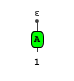
\includegraphics[scale=0.99]{obrazky/sxsx1.png}
}
\qquad
\subfloat[$T(2)$.]{
\label{img:sxsx2}
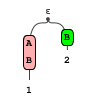
\includegraphics[scale=0.99]{obrazky/sxsx2.png}
}
\qquad
\subfloat[$T(3)$.]{
\label{img:sxsx3}
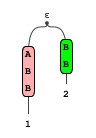
\includegraphics[scale=0.99]{obrazky/sxsx3.png}
}
% \qquad

\subfloat[$T(4)$.]{
\label{img:sxsx4}
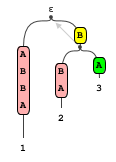
\includegraphics[scale=0.99]{obrazky/sxsx4.png}
}
\qquad
\subfloat[$T$.]{
\label{img:sxsx5}
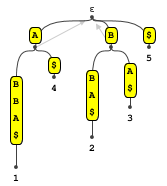
\includegraphics[scale=0.99]{obrazky/sxsx5.png}
}
\caption{\emph{Sufixové stromy.} Na obrázku sú sufixové stromy pre slová 
{\tt A}, {\tt AB}, {\tt ABB}, {\tt ABBA}, {\tt ABBA\uz}. Šípky znázorňujú 
sufixové linky, ružovou a zelenou sú označené hrany, na ktoré sa bude v 
nasledujúcom, kroku aplikovať prvé pravidlo. Čísla oznažujú, na ktorom znaku 
začína daný sufix v slove.}
\label{img:sxsx}
\end{figure}

\subsection{Zhrnutie}

Sufixový strom $T$ pre slovo $w = w_1w_2w_3\cdots w_n\uz$, vytvoríme tak, že z 
prázdneho stromu vytvoríme postupne stromy $T(1), T(2), T(3),\ldots, T(n), T$. 

Strom $T(1)$ vytvoríme triviálne; pridáme koreňu hranu s dvojicou indexov 
$(1, e)$ a nastavíme štartovací vrchol $u_s$ na práve vytvorený vrchol.

Postupne vytvárame strom $T(i)$ zo stromu $T(i-1)$ rozšírením stromu 
$T(i-1)$ o písmenko $w_i$\footnote{Respektíve strom $T$ zo stromu 
$T(n)$ o písmenko $w_n$.} nasledovne:

\begin{enumerate}
\item index $e$ nastavíme na novú hodnotu $i$; 
Tým sme vykonali všetky prvé prípady. Vieme si udržiavať ich počet $j$;
\item za aktuálny vrchol $u$ si zvolíme štartovací vrchol $u_s$;
\item z aktuálneho vrcholu prejdeme po hrane vyššie a zapamätáme si reťazec 
$\alpha$;
\item ak nie sme v koreni, prejdeme po sufixovom linku. Nastavíme aktuálny 
vrchol;
\item z aktuálneho vrcholu vyhľadáme reťazec $w_{j+1}\cdots w_i$;
\item teraz môže nastať druhý alebo tretí prípad:
\begin{itemize}
\item ak nastal druhý prípad, v prípade potreby rozdelíme hranu. Nastavíme 
aktuálny vrchol na posledný navštívený (respektíve vytvorený) a v prípade 
potreby nastavíme sufixový link. K aktívnemu vrcholu pripojíme hranu s 
indexami $(i,e)$, zvýšime index $j$ o 1 a nastavíme štartovací vrchol na 
práve vytvorený. Vrátime sa na krok~3;
\item ak nastal tretí prípad, v prípade potreby nastavíme sufixový link.
\end{itemize}
\item zvýšime hodnotu $i$ o jeden a vrátime sa na krok 1.
\end{enumerate}
 
Takto vybudujeme sufixový strom pre slovo $w$.

\section{Použitie}\label{sec:sx:usage}

Sufixový strom má v stringológií veľa využití
\citep{gusfield}. Najtriviálnejší je algoritmus na zistenie podreťazca v 
slove. Navyše vieme určiť, na ktore pozícií sa podreťazec vyskytuje. Pri 
konštrukcii stromu stačí označovať listy číslami v poradí podľa vytvorenia. 

Sufixový strom pre viacej reťazcov sa nazýva \emph{všeobecný sufixový strom} 
a dá sa zostrojiť miernou úpravou Ukkonenovho algoritmu. Reťazce $v_1, v_2, 
v_3, \ldots, v_n$ spojíme a oddelíme unikátnymi oddelovačmi. Vznikne nám slovo 
$v_1\uz_1v_2\uz_2v_3\uz_3\cdots v_n\uz_n$, z ktorého vieme vybudovať sufixový 
strom. Tento strom sa dá využiť na vyhľadanie najdlhšieho spoločného 
podreťazca. 

% \section{Vizualizácia}
% 
% Sufixový strom sme vizualizovali podobne ako písmenkový strom, použili sme 
% Walkerov algoritmus \citep{walker} so zakrivenými hranami. Sufixové linky 
% sme znázornili šedými šípkami. Na rozdiel od písmenkového stromu sa v 
% sufixovom strome vyskytujú na hranách reťazce. Tie sme znázornili ako viac 
% spojených hrán.
% 
% Pri vizualizácií algoritmu oznažujeme hrany, pre ktoré platí prvý prípad, 
% ružovou farbou. Hranu, pre ktorú platí prvý prípad a je pridaná ako posledná, 
% označujeme zelenou farbou. Z tejto hrany začína "zaujímavejšia" časť 
% rozširovania stromu.


